\documentclass[11pt,letterpaper]{article}

\usepackage[utf8]{inputenc}
\usepackage[margin=1in]{geometry}
\usepackage{amsmath, amssymb, amsthm, amsfonts}
\usepackage{graphicx}
\usepackage{xcolor}
\usepackage{hyperref}
\usepackage{booktabs}
\usepackage{cite}
\usepackage{titlesec}
\usepackage{tcolorbox}
\usepackage{float}
\usepackage{caption}
\usepackage{array}
\usepackage{enumitem}
\usepackage{siunitx}
\usepackage{kotex}
\usepackage{indentfirst}

\setlength{\parindent}{1.5em}
\setlength{\parskip}{0.25em}
\linespread{1.04}
\setcounter{tocdepth}{2}

\definecolor{ajpblue}{RGB}{28, 54, 115}
\definecolor{ajpsec}{RGB}{54, 95, 145}
\definecolor{bglight}{RGB}{245, 247, 250}
\definecolor{bordergrey}{RGB}{210, 215, 223}

\hypersetup{
colorlinks=true,
linkcolor=ajpblue,
citecolor=ajpsec,
urlcolor=ajpblue
}

\titleformat{\section}{\large\bfseries\color{ajpblue}}{\thesection}{1em}{}[{\titlerule[0.5pt]}]
\titleformat{\subsection}{\normalsize\bfseries\color{ajpsec}}{\thesubsection}{1em}{}
\titleformat{\subsubsection}{\normalsize\itshape\color{ajpsec}}{\thesubsubsection}{1em}{}

\newtcolorbox{physicsinsight}{
colback=bglight,
colframe=ajpsec,
boxrule=0.5pt,
left=3mm,
right=3mm,
top=2mm,
bottom=2mm,
arc=2pt
}

\graphicspath{{./}{Figure/}{figures/}}

\title{
\vspace{-1.5in}
\rule{\linewidth}{1.5pt} \\ \vspace{4mm}
\large\textbf{PHYSICS GROUP PROJECT REPORT} \\ \vspace{2mm}
\Large\textbf{Experimental and Computational Verification of \\ 
Gravitational Acceleration Measurement Using Bernoulli's Equation}
\\ \vspace{4mm}
\large\textit{Based on the Article ``Measurement of Gravitational Acceleration Using Bernoulli's Equation''} \\
\rule{\linewidth}{1.5pt}
}

\author{
\begin{tabular}{r @{\quad} p{5.0cm} @{\quad} l}
\textbf{Project Group:} & \multicolumn{2}{l}{[Hyunmin's Makchang / Group 13]} \\[1ex]
\textbf{Group Members:} 
& [곽민환(Kawak Minhwan)] & [202611011] \\
& [김하윤(Kim Hayun)] & [202611065] \\
& [박정환(Park Jeonghwan)] & [202611092] \\
& [신현민(Shin Hyunmin)] & [202611119] \\[1ex]
\textbf{Course Title:} & \multicolumn{2}{l}{[General Physics I]} \\
\textbf{Instructor:} & \multicolumn{2}{l}{[Prof. Deniz Olgu Devecioglu]} \\
\textbf{Section:} & \multicolumn{2}{l}{[04]}
\end{tabular}
}

\date{\today}

\begin{document}
\maketitle

\begin{abstract}
This project experimentally and computationally investigates the draining motion of water from a tank using Bernoulli's equation. The project is based on the article by Jang \textit{et al.}, ``Measurement of Gravitational Acceleration Using Bernoulli's Equation,'' published in \textit{The Physics Teacher} in 2024 \cite{jang2024}. In the present project, our group directly performed a draining-tank experiment, recorded the motion of the water, and analyzed the video using Tracker. From the Tracker analysis, time-dependent water-height and horizontal-reach data were obtained for five initial water-head conditions, $H_0=4,6,8,10,$ and $12~\mathrm{cm}$. In addition, a Python-based computer simulation was implemented from the Bernoulli draining model to predict the time evolution of the water head and the horizontal reach. The experimental results and simulation results were compared using linear regression and $R^2$ analysis. The linearized water-height variable $\sqrt{H(t)}$ showed strong agreement with the Bernoulli prediction, with an average coefficient of determination of approximately $\bar{R}^2=0.986$. The horizontal reach $x_R(t)$ also showed approximate linear behavior, with $\bar{R}^2=0.977$, but it was more sensitive to jet spreading and endpoint-selection uncertainty. These results show that both the direct experiment and the computer simulation support the Bernoulli-based linear model.
\end{abstract}

\begin{center}
\textbf{Project Repository:} \\
\url{https://github.com/houar1223/General_Physics_1_Project.git}
\end{center}

\newpage
\tableofcontents
\newpage

% =========================================================================
\section{Introduction}
% =========================================================================

The acceleration due to gravity is commonly measured through free-fall, projectile-motion, or pendulum experiments. These methods usually involve solid objects moving under gravity. However, gravity also appears in fluid motion. When water drains from a side hole in a tank, gravitational potential energy associated with the water height is converted into kinetic energy of the water jet. Therefore, the draining motion of water can provide another way to study gravitational acceleration and energy conversion.

The article by Jang \textit{et al.} proposed a method for estimating gravitational acceleration using Bernoulli's equation \cite{jang2024}. Their study analyzed two measurable quantities: the decrease of water height in a tank and the horizontal reach of a water jet. Both quantities were converted into linear graph relationships whose slopes can be connected to $g$ if the apparatus constants are known.

In this project, our group reproduced the main idea of the article through both direct experimentation and computer simulation. First, we performed an actual draining-tank experiment and recorded the motion of the water. The recorded video was analyzed using Tracker, and the measured values of water height and horizontal reach were obtained from the video. Second, we used Python to simulate the draining process from the Bernoulli-based model. Finally, the experimental results, the regression results, and the simulation trends were compared.

The main research question is whether the directly measured Tracker data and the Bernoulli-based simulation show the same linear relationships predicted by theory. Specifically, we tested whether $\sqrt{H(t)}$ decreases linearly with time and whether the horizontal reach $x_R(t)$ also decreases approximately linearly.

% =========================================================================
\section{Theory and Model Derivation}
% =========================================================================

\subsection{Bernoulli's Equation and Torricelli's Law}

Bernoulli's equation expresses conservation of mechanical energy along a streamline for steady, incompressible, and non-viscous flow:
\begin{equation}
    P+\rho gh+\frac{1}{2}\rho v^2=\text{constant}.
    \label{eq:bernoulli_general}
\end{equation}
Here, $P$ is pressure, $\rho$ is fluid density, $g$ is gravitational acceleration, $h$ is height, and $v$ is fluid speed. Applying Eq.~\eqref{eq:bernoulli_general} between the water surface and the outlet gives
\begin{equation}
    P_0+\rho gh_0+\frac{1}{2}\rho v_0^2
    =
    P_a+\rho gh_a+\frac{1}{2}\rho v_a^2.
    \label{eq:bernoulli_points}
\end{equation}
Since both points are exposed to atmospheric pressure, $P_0=P_a$. Also, because the tank area is much larger than the outlet area, the water surface speed is much smaller than the outlet speed, so $v_0\approx0$. Therefore,
\begin{equation}
    \rho gh_0=\rho gh_a+\frac{1}{2}\rho v_a^2.
\end{equation}
After canceling $\rho$ and defining the water head above the outlet as
\begin{equation}
    H(t)=h(t)-h_a,
\end{equation}
the ideal outlet speed becomes
\begin{equation}
    v_a(t)=\sqrt{2gH(t)}.
    \label{eq:torricelli}
\end{equation}

This result is Torricelli's law. It shows that the exit speed is determined by the water head above the outlet.

\subsection{Hydraulic Coefficients}

The ideal model does not fully describe real water flow. The stream contracts after leaving the hole, and viscous effects reduce the actual jet speed. These effects are represented by hydraulic coefficients. If $A_b$ is the geometric outlet area and $A_a$ is the effective jet area, then
\begin{equation}
    A_a=c_cA_b,
\end{equation}
where $c_c$ is the contraction coefficient. The real velocity is written as
\begin{equation}
    v_{\text{real}}=c_vv_a,
\end{equation}
where $c_v$ is the velocity coefficient. The volume flow rate becomes
\begin{equation}
    Q=A_av_{\text{real}}=c_cc_vA_bv_a.
\end{equation}
The discharge coefficient is defined as
\begin{equation}
    c_d=c_cc_v,
\end{equation}
so the flow rate is
\begin{equation}
    Q=c_dA_b\sqrt{2gH}.
    \label{eq:flowrate}
\end{equation}

The coefficients $c_d$, $c_v$, and $c_c$ depend on outlet shape, wall thickness, water head, and flow condition. Therefore, an assumed coefficient can introduce systematic error even when the graph is linear.

\subsection{Water-Height Linear Model}

As water drains from the tank, the water head decreases. If the tank cross-sectional area is $A_0$, a small decrease $dH$ corresponds to a discharged volume
\begin{equation}
    dV_{\text{out}}=-A_0\,dH.
\end{equation}
The same volume can be written as $Qdt$. Using Eq.~\eqref{eq:flowrate},
\begin{equation}
    -A_0\,dH=c_dA_b\sqrt{2gH}\,dt.
\end{equation}
Rearranging and integrating from $H_0$ at $t=0$ to $H(t)$ at time $t$ gives
\begin{equation}
    \sqrt{H(t)}
    =
    \sqrt{H_0}
    -
    \frac{c_dA_b}{A_0}\sqrt{\frac{g}{2}}\,t.
    \label{eq:height_model}
\end{equation}
Thus, $\sqrt{H(t)}$ should be a linear function of time. The slope is
\begin{equation}
    k_1=-\frac{c_dA_b}{A_0}\sqrt{\frac{g}{2}}.
    \label{eq:k1}
\end{equation}
If the apparatus constants are known, the gravitational acceleration can be calculated from
\begin{equation}
    g=2\left(\frac{|k_1|A_0}{c_dA_b}\right)^2.
    \label{eq:g_method1}
\end{equation}

\subsection{Horizontal-Reach Linear Model}

After leaving the side outlet, the water jet moves approximately as a horizontally launched projectile. If the vertical distance from the outlet to the landing surface is $h_a$, the time of flight is
\begin{equation}
    t_f=\sqrt{\frac{2h_a}{g}}.
\end{equation}
The horizontal reach is
\begin{equation}
    x_R=v_{\text{real}}t_f.
\end{equation}
Using $v_{\text{real}}=c_v\sqrt{2gH}$,
\begin{equation}
    x_R=2c_v\sqrt{Hh_a}.
    \label{eq:xR_H}
\end{equation}
Substituting Eq.~\eqref{eq:height_model} into Eq.~\eqref{eq:xR_H} gives
\begin{equation}
    x_R(t)=2c_v\sqrt{H_0h_a}
    -
    \frac{c_vc_dA_b}{A_0}\sqrt{2gh_a}\,t.
    \label{eq:reach_model}
\end{equation}
Therefore, $x_R(t)$ should also decrease approximately linearly with time. The slope is
\begin{equation}
    k_2=-\frac{c_vc_dA_b}{A_0}\sqrt{2gh_a}.
\end{equation}

\begin{physicsinsight}
The height model directly tests the draining process, while the reach model combines draining flow with projectile motion. For this reason, the height model is usually more stable, and the reach model is more sensitive to endpoint measurement error.
\end{physicsinsight}

% =========================================================================
\section{Actual Experiment and Tracker Measurement}
% =========================================================================

\subsection{Experimental Setup}

The experiment was directly performed by our group. A water tank with a side outlet was prepared, and water was filled to selected initial heights above the outlet. After the outlet was opened, water drained from the tank and formed a horizontal jet. The process was recorded using a camera or smartphone so that the water height and jet reach could be analyzed frame by frame.

\begin{figure}[H]
\centering
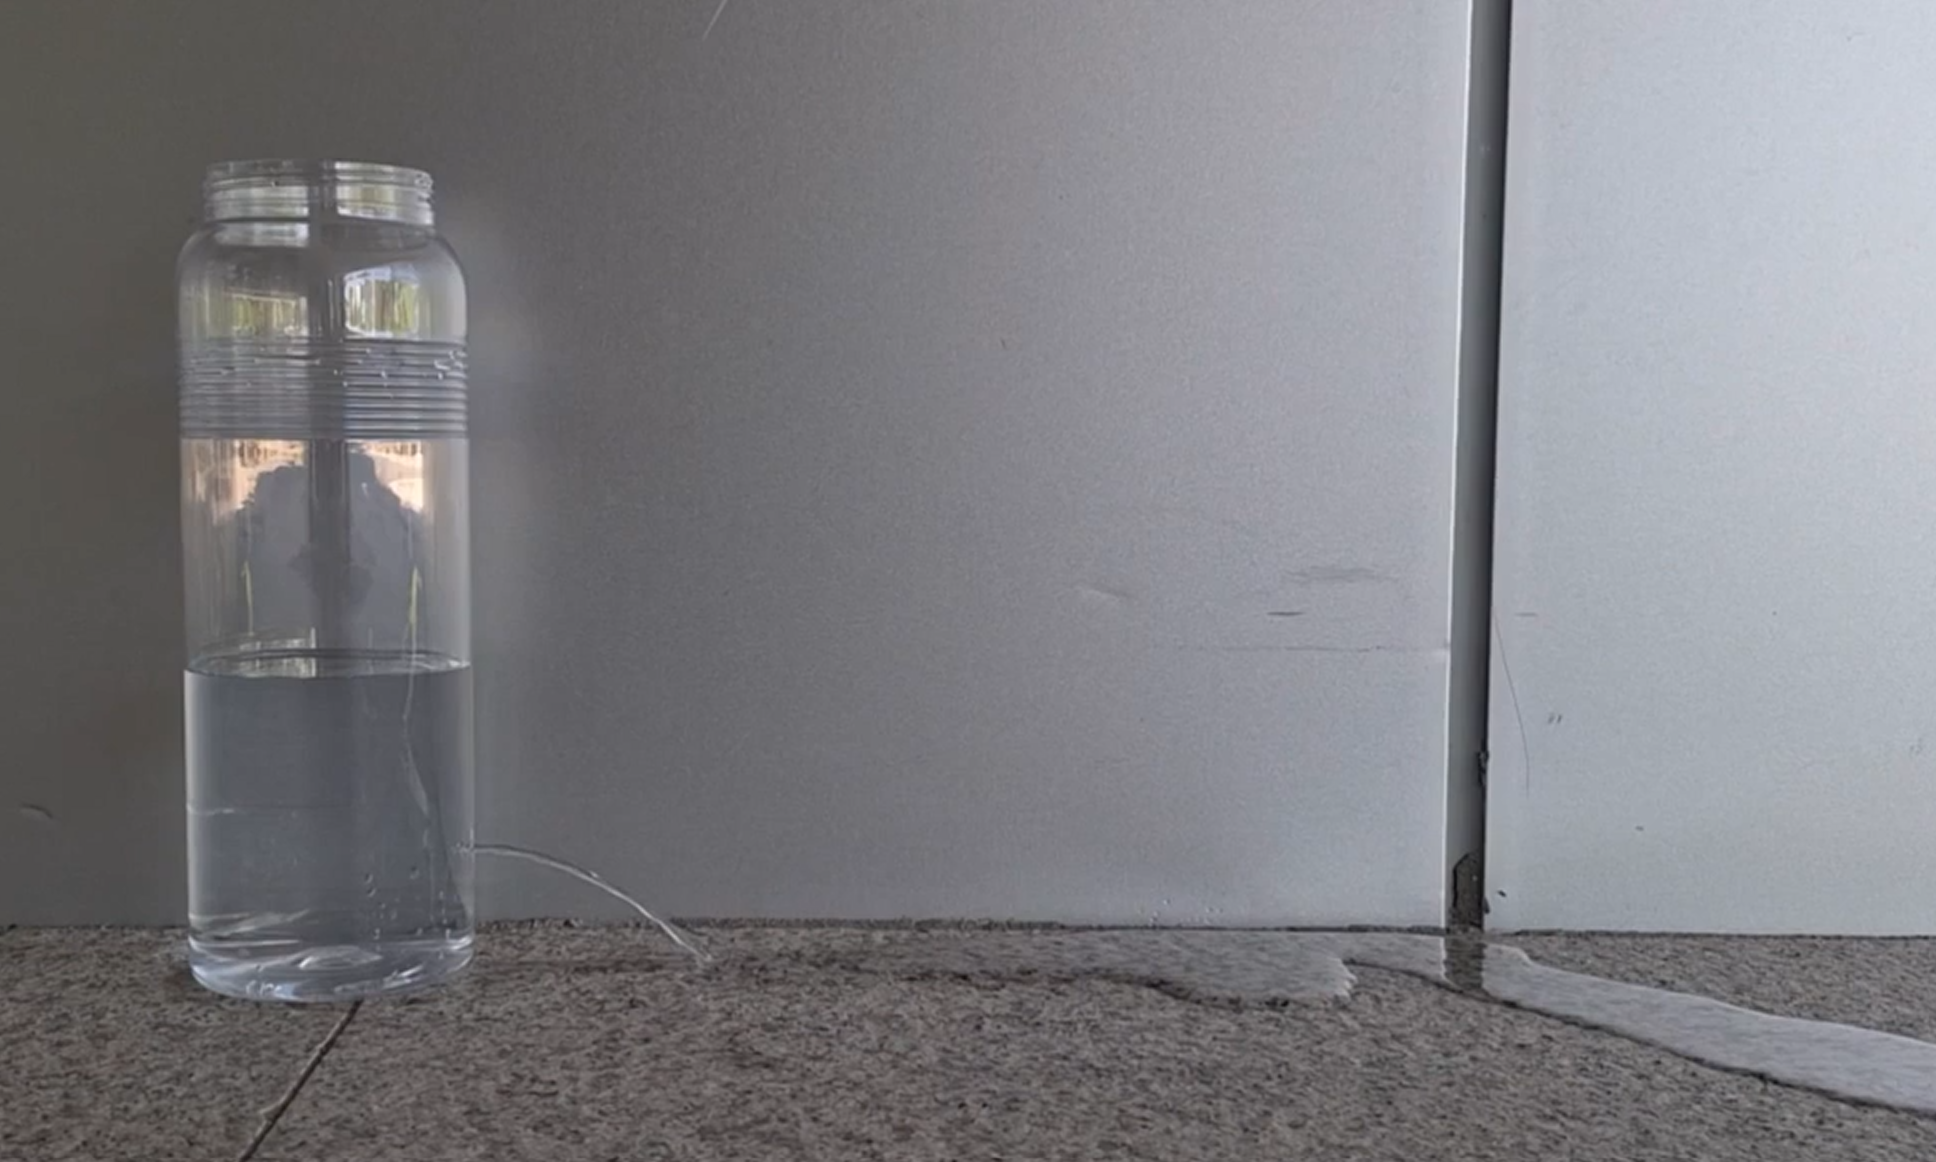
\includegraphics[width=0.62\linewidth]{Experiment.png}
\caption{Actual apparatus used for the draining-tank experiment.}
\label{fig:apparatus}
\end{figure}

The initial water-head conditions were
\begin{equation}
    H_0=4,6,8,10,12~\mathrm{cm}.
\end{equation}

These five conditions allowed the model to be tested over several pressure-head values. A larger initial head should produce a faster initial jet and a longer horizontal reach, while a smaller head should produce a weaker jet.

\subsection{Tracker Data Extraction}

After the experiment was recorded, the video was analyzed using Tracker. A calibration scale was set in the video, and the relevant positions were measured at selected time intervals. The two main quantities extracted from Tracker were the water-surface height and the horizontal reach of the water jet.

\begin{figure}[H]
\centering
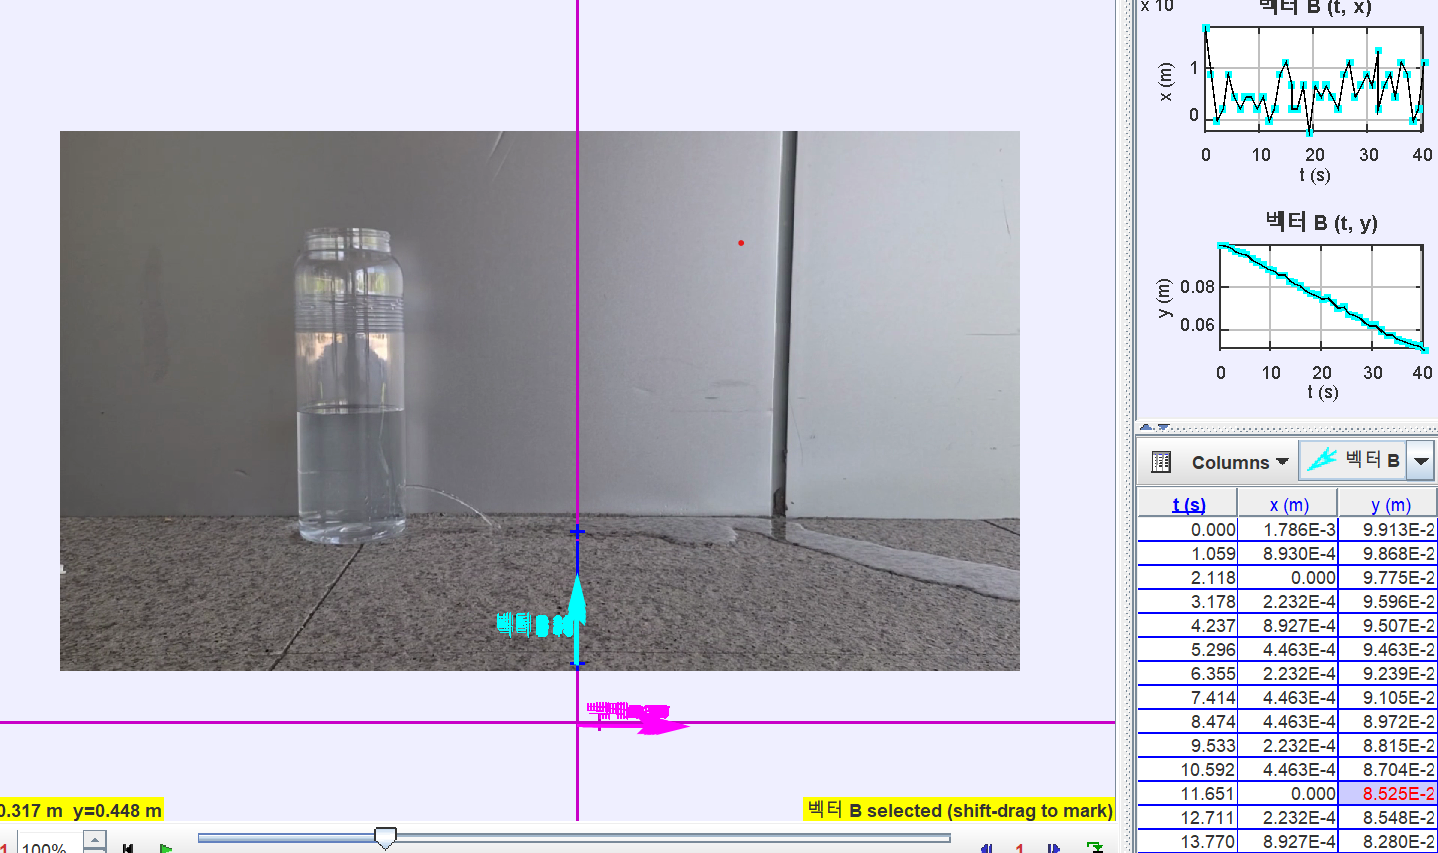
\includegraphics[width=0.78\linewidth]{Tracker.png}
\caption{Tracker video-analysis process used to extract experimental data from the recorded experiment.}
\label{fig:tracker}
\end{figure}

The data used in the analysis were obtained from the actual experiment through Tracker. The measurements were grouped according to the five initial water-head conditions, $H_0=4,6,8,10,$ and $12~\mathrm{cm}$. For each condition, the experimental results included time, horizontal reach, and water-surface height. These measured values served as the experimental basis for the Python analysis and simulation comparison.

\begin{table}[H]
\centering
\caption{Main symbols used in the experiment and analysis.}
\label{tab:variables}
\begin{tabular}{lll}
\toprule
\textbf{Symbol} & \textbf{Physical meaning} & \textbf{Unit} \\
\midrule
$g$ & Gravitational acceleration & $\mathrm{m/s^2}$ \\
$H(t)$ & Water head above the outlet from Tracker data & $\mathrm{m}$ \\
$H_0$ & Initial water head above the outlet & $\mathrm{m}$ \\
$x_R(t)$ & Horizontal reach from Tracker data & $\mathrm{m}$ or $\mathrm{cm}$ \\
$A_0$ & Cross-sectional area of the tank & $\mathrm{m^2}$ \\
$A_b$ & Area of the outlet hole & $\mathrm{m^2}$ \\
$c_d$ & Discharge coefficient & dimensionless \\
$c_v$ & Velocity coefficient & dimensionless \\
$t$ & Time after opening the outlet & $\mathrm{s}$ \\
\bottomrule
\end{tabular}
\end{table}

% =========================================================================
\section{Computer Simulation and Python Analysis}
% =========================================================================

\subsection{Simulation Model}

A computer simulation was used to calculate the theoretical motion predicted by the Bernoulli model. The simulation was not a replacement for the actual experiment; it was used as a comparison tool. The experiment provided measured data from Tracker, while the simulation provided the ideal model-based trend.

The simulation used the differential equation
\begin{equation}
    \frac{dH}{dt}
    =
    -\frac{c_dA_b}{A_0}\sqrt{2gH}.
    \label{eq:simulation_ode}
\end{equation}

For numerical updating with time step $\Delta t$,
\begin{equation}
    H_{n+1}
    =
    H_n
    -
    \frac{c_dA_b}{A_0}\sqrt{2gH_n}\Delta t.
    \label{eq:euler_update}
\end{equation}
After calculating $H_n$, the corresponding horizontal reach was predicted using
\begin{equation}
    x_{R,n}=2c_v\sqrt{H_nh_a}.
    \label{eq:sim_reach}
\end{equation}

This procedure generated theoretical curves for $H(t)$ and $x_R(t)$.

\subsection{Python Workflow}

Python was used for both simulation and regression analysis. The workflow was:
\begin{enumerate}[itemsep=0.1em]
    \item organize the Tracker-based experimental measurements by initial water-head condition;
    \item read the measured time, horizontal reach, and water-surface height values;
    \item convert units where necessary;
    \item compute $\sqrt{H(t)}$;
    \item simulate $H(t)$ and $x_R(t)$ from the Bernoulli model;
    \item fit $\sqrt{H(t)}=a_1+k_1t$ and $x_R(t)=a_2+k_2t$;
    \item calculate $R^2$ values and generate graphs.
\end{enumerate}
The coefficient of determination was calculated as
\begin{equation}
    R^2=1-\frac{\sum_i(y_i-\hat{y}_i)^2}{\sum_i(y_i-\bar{y})^2}.
\end{equation}

A value of $R^2$ close to 1 means that the measured data follow the fitted line closely.

% =========================================================================
\section{Results}
% =========================================================================

\subsection{Horizontal Reach from Tracker Data}

Figure~\ref{fig:reach} shows the horizontal reach $x_R(t)$ obtained from Tracker analysis for the five initial water-head conditions. The reach generally decreased as time increased, which agrees with the expectation that the jet becomes slower as the water level decreases.

\begin{figure}[H]
\centering
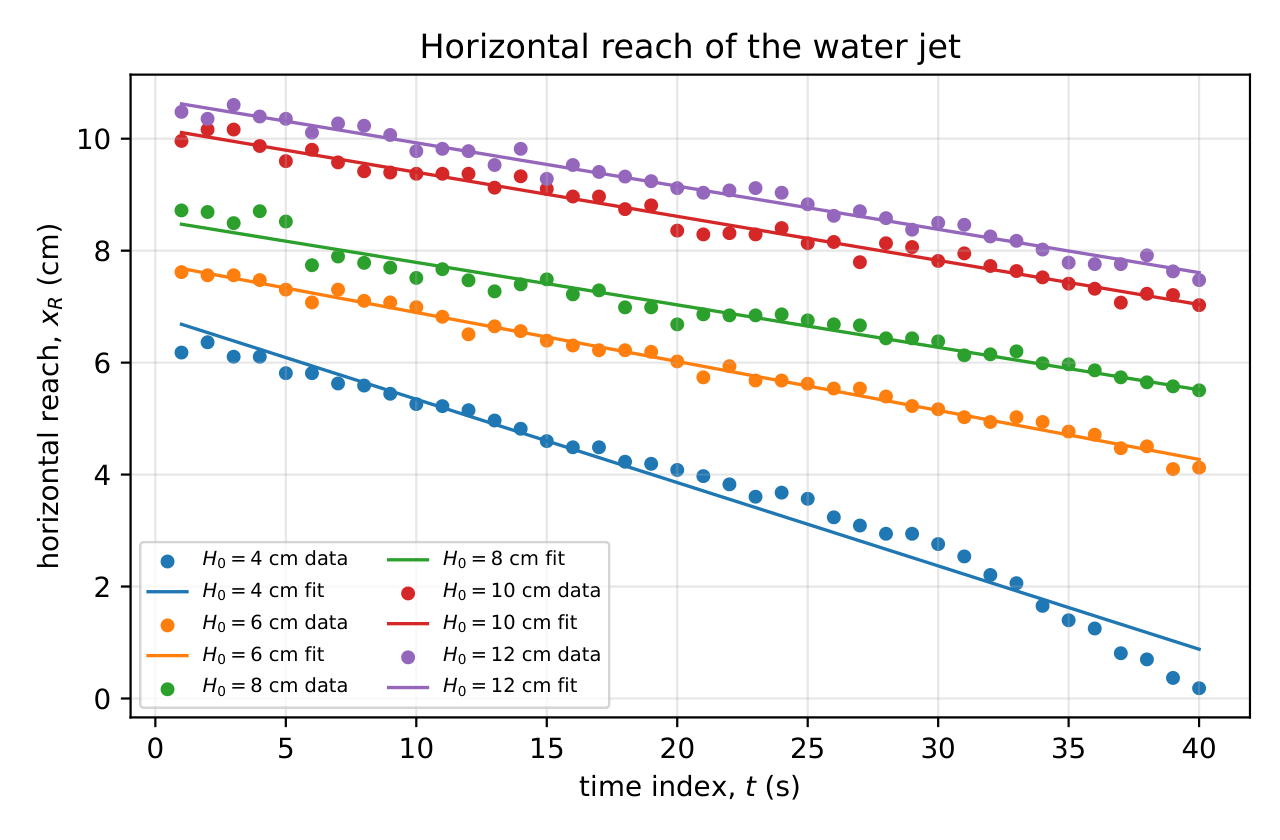
\includegraphics[width=0.72\linewidth]{fig_reach_vs_time.png}
\caption{Horizontal reach $x_R(t)$ of the water jet measured from Tracker data.}
\label{fig:reach}
\end{figure}

The horizontal-reach data showed approximate linear behavior, but the scatter was larger than in the height analysis. This is reasonable because the endpoint of the jet is difficult to define precisely. The stream spreads and can break into droplets, especially when the water head becomes small.

\subsection{Linearized Water-Height Data}

Figure~\ref{fig:sqrth} shows $\sqrt{H(t)}$ calculated from the Tracker-measured water-surface height. According to Eq.~\eqref{eq:height_model}, this quantity should decrease linearly with time.

\begin{figure}[H]
\centering
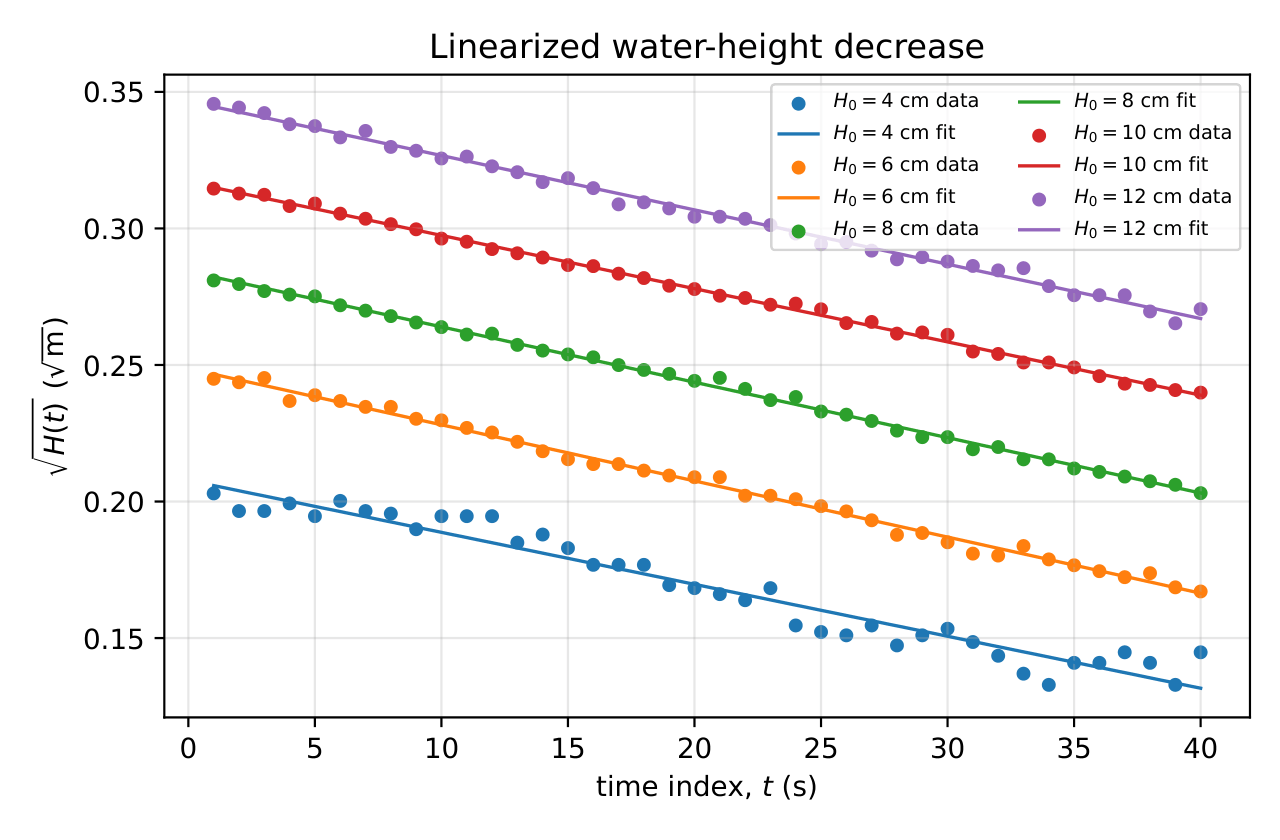
\includegraphics[width=0.84\linewidth]{fig_sqrt_height_vs_time.png}
\caption{Linearized water-height decrease calculated from Tracker measurements.}
\label{fig:sqrth}
\end{figure}

The linearized height data followed straight lines closely for all five initial height conditions. The average $R^2$ value was approximately 0.986, indicating strong agreement with the Bernoulli-based model. Compared with the reach data, the height data produced a more stable and consistent linear relation.

\subsection{Regression Summary}

Table~\ref{tab:fit_summary} summarizes the regression results obtained from the Python analysis of the Tracker-based experimental data.

\begin{table}[H]
\centering
\caption{Linear-fit summary from Python analysis of Tracker-based data.}
\label{tab:fit_summary}
\small
\begin{tabular}{@{}rrrrrrr@{}}
\toprule
$H_0$ & $k_2$ & $R^2_x$ & $10^3k_1$ & $R^2_H$ & $h_a$ & $A_0/A_b$ \\
(cm) & (cm/s) & & ($\sqrt{\mathrm{m}}$/s) & & (cm) & calibrated \\
\midrule
4  & -0.1488 & 0.972 & -1.903 & 0.945 & 3.04 & 710 \\
6  & -0.0875 & 0.991 & -2.056 & 0.994 & 2.62 & 657 \\
8  & -0.0759 & 0.961 & -2.029 & 0.998 & 2.38 & 666 \\
10 & -0.0788 & 0.980 & -1.950 & 0.998 & 2.70 & 693 \\
12 & -0.0773 & 0.983 & -1.989 & 0.994 & 2.48 & 679 \\
\bottomrule
\end{tabular}
\end{table}

The fitted slopes of $\sqrt{H(t)}$ were clustered around
\begin{equation}
    k_1\approx -1.99\times 10^{-3}~\sqrt{\mathrm{m}}/\mathrm{s}.
\end{equation}

This consistency is important because the theoretical slope should depend mainly on the outlet geometry, tank geometry, discharge coefficient, and gravitational acceleration, rather than on the initial water head. The horizontal-reach slopes showed larger variation, especially for $H_0=4~\mathrm{cm}$, suggesting stronger endpoint uncertainty at low head.

\subsection{Intercept Scaling and Simulation Consistency}

The horizontal-reach model predicts that the initial reach should scale with $\sqrt{H_0}$:
\begin{equation}
    x_R(0)=2c_v\sqrt{H_0h_a}.
\end{equation}

Therefore, the fitted intercept of $x_R(t)$ should be approximately proportional to $\sqrt{H_0}$.

\begin{figure}[H]
\centering
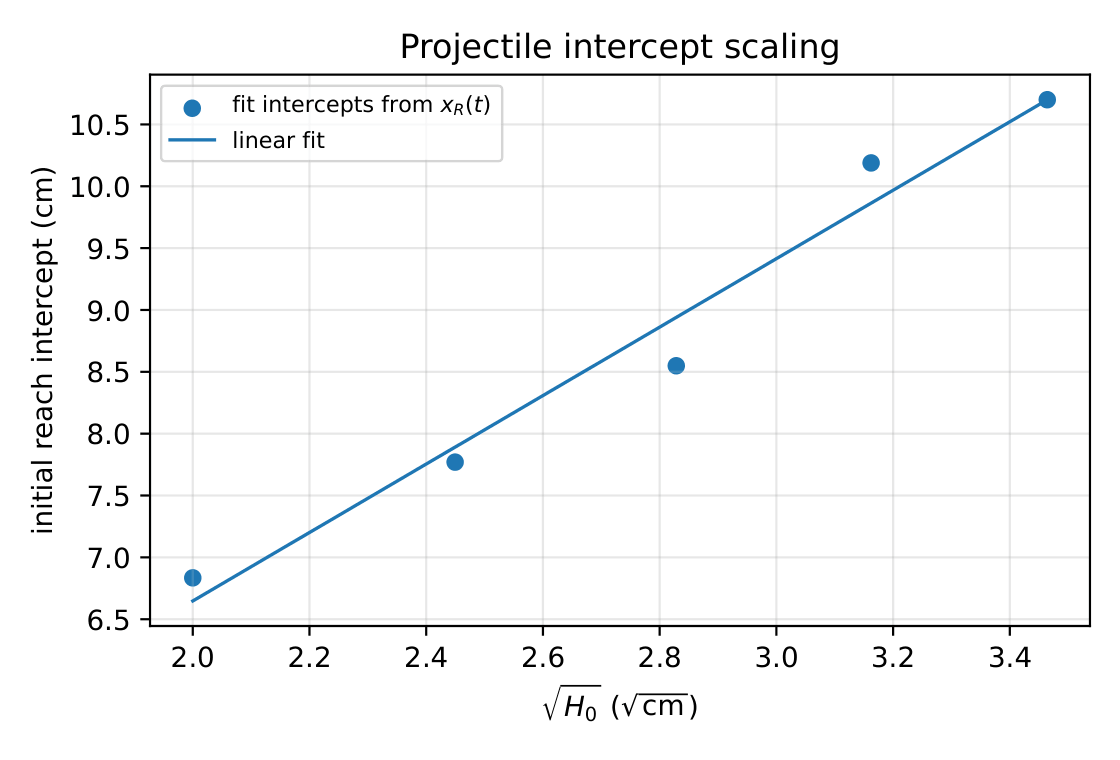
\includegraphics[width=0.64\linewidth,height=0.25\textheight,keepaspectratio]{fig_intercept_scaling.png}
\caption{Scaling of the fitted horizontal-reach intercept with $\sqrt{H_0}$.}
\label{fig:intercept}
\end{figure}

The intercept-based estimate of the outlet-to-landing height was approximately
\begin{equation}
    h_a=2.64\pm0.25~\mathrm{cm}
\end{equation}
when all five conditions were included. When the lowest-head condition was excluded, the estimate became
\begin{equation}
    h_a=2.55\pm0.14~\mathrm{cm}.
\end{equation}

The smaller uncertainty after excluding the lowest-head condition supports the interpretation that low-head data were more sensitive to jet instability and Tracker endpoint-selection uncertainty.

The computer simulation showed the same qualitative tendency as the experiment. As the water head decreased, the predicted water-jet reach also decreased. The simulation also reproduced the key linearized relationship between $\sqrt{H(t)}$ and time. Therefore, the simulation and the experiment both support the same Bernoulli-based interpretation.

% =========================================================================
\section{Discussion}
% =========================================================================

\subsection{Theory, Simulation, and Experiment}

The theoretical model predicted that $\sqrt{H(t)}$ should decrease linearly with time and that $x_R(t)$ should also decrease approximately linearly. The simulation followed directly from these equations and provided a clean model prediction. The actual experiment, analyzed through Tracker, tested whether real water motion followed the same behavior.

The results showed that the experiment and simulation agreed in their overall trends. The water-height data had strong linearity, indicating that the draining process was well described by the Bernoulli model. The horizontal-reach data were also approximately linear, but less stable. This agrees with the reference article, which also concluded that the water-height method is generally more accurate than the horizontal-reach method \cite{jang2024}.

\subsection{Reliability of the Height Method}

The water-height method was more reliable because the water surface is broad and moves relatively slowly, making it easier to track in Tracker. The transformation $\sqrt{H(t)}$ also directly linearizes the draining equation. In contrast, the horizontal-reach method depends on identifying the endpoint of a moving and spreading water jet. At low water head, the jet becomes weaker and can break into droplets, making the measured reach more subjective.

\subsection{Effective Area Ratio}

Using $g_0=9.80665~\mathrm{m/s^2}$ and assuming $c_d=0.61$, the fitted water-height slopes imply an effective area ratio of approximately
\begin{equation}
    \frac{A_0}{A_b}=681\pm21.
\end{equation}

This value should be interpreted as a calibrated effective ratio rather than a direct geometric measurement. If the actual tank diameter $D_0$ and outlet diameter $D_b$ are known, the geometric ratio can be calculated as
\begin{equation}
    \frac{A_0}{A_b}
    =
    \left(\frac{D_0}{D_b}\right)^2.
\end{equation}

Comparing the geometric ratio with the calibrated ratio would be useful for evaluating the apparatus.

\subsection{Sources of Error and Improvements}

Several sources of error likely affected the experiment. Tracker calibration uncertainty could create systematic error in both height and reach measurements. Camera parallax could distort the measured positions if the camera was not perpendicular to the measurement plane. Jet spreading made the endpoint difficult to determine, especially at low water head. Water-surface oscillation after opening the outlet could also affect the height measurement. In addition, the discharge coefficient depends on the actual outlet geometry and flow condition, and the simulation did not fully include turbulence, splash formation, air resistance, or detailed viscous losses.

The experiment could be improved by measuring the tank diameter, outlet diameter, outlet height, and landing height with uncertainties. The camera should be fixed on a tripod and aligned perpendicular to the measurement plane. A ruler or calibration grid should be placed in the same plane as the water jet. Repeated trials should be performed for each initial height. The Tracker analysis could also be improved by using a consistent rule for selecting the jet endpoint, such as tracking the center of the main impact region rather than the farthest visible droplet.

% =========================================================================
\section{Conclusion}
% =========================================================================

This project analyzed the draining motion of water from a tank using Bernoulli's equation, Tracker-based experimental measurement, and computer simulation. Our group directly performed the experiment, recorded the water motion, extracted data using Tracker, and analyzed the experimental results using Python. A computer simulation based on the Bernoulli draining model was also used to calculate the expected time evolution of the water head and horizontal reach.

The theoretical model predicted that $\sqrt{H(t)}$ should decrease linearly with time and that $x_R(t)$ should also decrease approximately linearly. The Tracker-based experimental results supported these predictions. The linearized water-height method showed strong agreement with the model, with an average $R^2$ value of approximately 0.986. The horizontal-reach method also showed approximate linearity, with an average $R^2$ value of approximately 0.977, but it was more affected by jet spreading and endpoint-selection uncertainty.

The computer simulation and the actual experiment showed the same overall physical trend: as the water head decreased, the water jet became weaker and the horizontal reach decreased. This agreement supports the Bernoulli-based interpretation that gravitational potential energy is converted into kinetic energy of the water jet. Overall, the project confirms that gravitational effects can be studied through fluid motion, not only through the motion of solid objects. However, a more accurate numerical measurement of $g$ would require more precise calibration of the tank area, outlet area, outlet-to-landing height, discharge coefficient, and time interval.

% =========================================================================
\begin{thebibliography}{99}
% =========================================================================

\bibitem{jang2024}
T. Jang, S. H. Sohn, H. Ha, S. Kwon, G. Lee, D. Lee, Y. Lee, S. W. Park, J. Y. Jang, J. Kim, S. E. Kwak, and J. Kim,
``Measurement of Gravitational Acceleration Using Bernoulli's Equation,''
\textit{The Physics Teacher}, vol. 62, no. 4, pp. 268--271, Apr. 2024. \url{https://doi.org/10.1119/5.0118197}

\bibitem{halliday2014}
D. Halliday, R. Resnick, and J. Walker,
\textit{Principles of Physics},
10th ed. John Wiley \& Sons, 2014.

\bibitem{saleta2005}
M. E. Saleta, D. Tobia, and S. Gil,
``Experimental Study of Bernoulli's Equation with Losses,''
\textit{American Journal of Physics}, vol. 73, no. 7, pp. 598--602, Jul. 2005. \url{https://doi.org/10.1119/1.1858486}

\bibitem{lienhard1984}
J. H. Lienhard V and J. H. Lienhard IV,
``Velocity Coefficients for Free Jets From Sharp-Edged Orifices,''
\textit{Journal of Fluids Engineering}, vol. 106, no. 1, pp. 13--17, Mar. 1984. \url{https://doi.org/10.1115/1.3242391}

\end{thebibliography}

\end{document}